\documentclass[tikz, border=10pt]{standalone}
\usetikzlibrary{arrows.meta, positioning, backgrounds}

\begin{document}
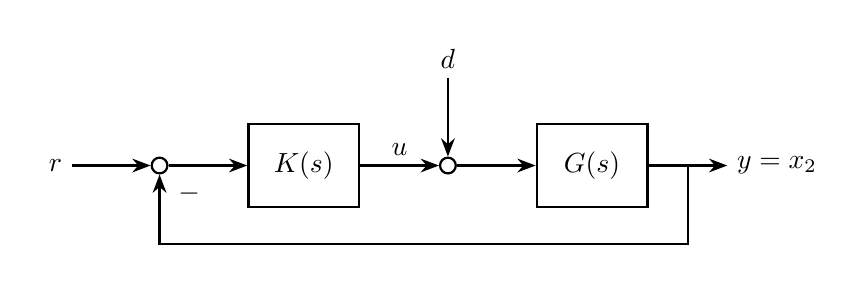
\begin{tikzpicture}[
	background rectangle/.style={fill=white},
    show background rectangle,
    % Styles for blocks and arrows
    block/.style={draw, rectangle, minimum height=3em, minimum width=4em, thick},
    sum/.style={draw, circle, inner sep=0pt, minimum size=2mm, thick},
    connector/.style={-Stealth, thick}
]

    % --- NODES ---
    % Starting from left to right
    \node (input) {$r$};
    \node [sum, right=of input] (sum1) {};
    \node [block, right=of sum1] (controller) {$K(s)$};
    \node [sum, right=of controller] (sum2) {};
    \node [block, right=of sum2] (plant) {$G(s)$};
    \node [right=of plant] (output) {$y = x_2$};
    
    % Disturbance node
    \node [above=of sum2] (dist) {$d$};

    % --- CONNECTIONS ---
    % Forward path
    \draw [connector] (input) -- (sum1);
    \draw [connector] (sum1) -- (controller) node[midway, above] {};
    \draw [connector] (controller) -- (sum2) node[midway, above] {$u$};
    \draw [connector] (sum2) -- (plant);
    \draw [connector] (plant) -- (output);
    
    % Disturbance path
    \draw [connector] (dist) -- (sum2);

    % Feedback path
    \draw [connector] (plant.east) -- ++(0.5,0) -- ++(0,-1.0) -| (sum1.south) {};

    % Labels for the sum nodes
    \node [below right=0.05cm of sum1] {$-$};

\end{tikzpicture}
\end{document}